\apendice{Especificación de Requisitos}

\section{Introducción}
Para poder llevar a cabo un proyecto de \textit{sofware}, se necesitan tener requisitos especificados, con esto se podrá realizar el desarrollo, usando estos requisitos como guía.

En este apartado se van a abarcar las especificaciones de requisitos y los casos de uso que reflejarán el funcionamiento del producto de \textit{software} desarrollado.

\section{Objetivos generales}
Este proyecto tiene como objetivo principal la generación de laberintos que puedan ser navegables por el usuario. Los objetivos para llevar a cabo el proyecto son los siguientes:
\begin{enumerate}
    \item Obtener laberintos que sean navegables.
    \item Utilizar varios algoritmos de generación procedimental para generar los laberintos.
    \item Usar la arquitectura cliente-servidor para poder almacenar datos del videojuego.
    \item Utilizar el protocolo HTTP para que el servidor se comunique con Unity.
    \item Calcular los tiempos de ejecución de estos algoritmos y compararlos.
    \item Generar una imagen del contenido con Docker para que se pueda alojar fácilmente en un servidor externo.
\end{enumerate}


\section{Catalogo de requisitos}

\subsection{Requisitos funcionales}
Los requisitos funcionales definen el comportamiento que se espera por la aplicación. Para este proyecto se han redactado los siguientes:

%    \item \textbf{RF1 - }
%		\begin{itemize}
%  			\item \textbf{RF1.1}: 
%			\item \textbf{RF1.2}: 
%			\item \textbf{RF1.3}:
%		\end{itemize}

\begin{itemize}
	\item \textbf{RF1 - Laberintos navegables}
		\begin{itemize}
  			\item \textbf{RF1.1}: El usuario puede navegar por el laberinto con el objeto <<Player>> utilizando las teclas W, A, S, D.
            \item \textbf{RF1.2}: El usuario colisiona con los muros, es decir, no puede atravesar paredes.
			\item \textbf{RF1.3}: El usuario puede tener acceso a la pantalla anterior con un botón de retorno.
            \item \textbg{RF1.4}:
		\end{itemize}
    \item \textbf{RF2 - Gestión del menú principal}
		\begin{itemize}
  			\item \textbf{RF2.1}: El usuario puede navegar por el menú principal
			\item \textbf{RF2.2}: El usuario puede abandonar el juego.
			\item \textbf{RF2.3}: El usuario puede moverse a la siguiente pantalla a través del menú.
		\end{itemize}
    \item \textbf{RF3 - Gestión del menú secundario}
		\begin{itemize}
  			\item \textbf{RF3.1}: El usuario puede navegar el menú secundario.
			\item \textbf{RF3.2}: El usuario puede seleccionar el algoritmo que desea usar para la generación del laberinto.
			\item \textbf{RF3.3}: El usuario debe poder acceso a la pantalla anterior con un botón de retorno.
		\end{itemize}
    \item \textbf{RF4 - Gestión de los laberintos generados}
		\begin{itemize}
  			\item \textbf{RF4.1}: La aplicación puede almacenar los laberintos con sus dimensiones y  semilla generados.
		\end{itemize}
    \item \textbf{RF5 - Generación de laberintos parametrizables}
		\begin{itemize}
  			\item \textbf{RF5.1}: El usuario puede introducir el ancho del laberinto a generar si el algoritmo lo permite.
            \item \textbf{RF5.2}: El usuario puede introducir el largo del laberinto a generar si el algoritmo lo permite.
            \item \textbf{RF5.3}: El usuario puede introducir el número de iteraciones si el algoritmo lo permite.
            \item \textbf{RF5.4}: El usuario puede introducir la semilla de la generación procedimental.
		\end{itemize}
\end{itemize}

\subsection{Requisitos no funcionales}
Los requisitos no funcionales engloban aquellos que no especifican el funcionamiento de la aplicación, van a definir el comportamiento del producto.
\begin{itemize}
    \item \textbf{RNF1 - Velocidad de respuesta}
		\begin{itemize}
  			\item \textbf{RNF1.1}: La carga del laberinto debe ser lo más rápida posible.
		\end{itemize}
    \item \textbf{RNF2 - Transparencia}
		\begin{itemize}
  			\item \textbf{RNF2.1}: Los cambios futuros deberán ser transparentes al usuario, ya que no hay necesidad de que conozca cómo funciona internamente el programa
		\end{itemize}
    \item \textbf{RNF3 - Usabilidad}
		\begin{itemize}
  			\item \textbf{RNF3.1}: La navegación por la aplicación debe de ser cómoda.
            \item \textbf{RNF3.2}: La navegación por los laberintos debe de ser intuitiva.
		\end{itemize}
\end{itemize}


\section{Especificación de requisitos}
\begin{figure}[!h]  
    \centering  
    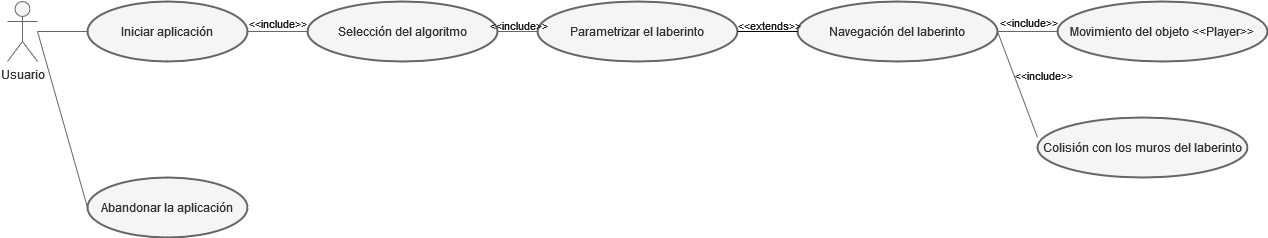
\includegraphics[width=\textwidth]{img/CasosUso.png}  
    \caption{Caso de uso de la aplicación.}  
    \label{fig:CasosDeUso}
\end{figure}
\begin{table}[p]
	\centering
	\begin{tabularx}{\linewidth}{ p{0.21\columnwidth} p{0.71\columnwidth} }
			\toprule
			\textbf{CU-1}    & \textbf{Iniciar aplicación}\\
			\toprule
			\textbf{Versión}              & 1.0    \\
			\textbf{Autor}                & Elsa Tolín \\
			\textbf{Requisitos asociados} & RF-2.1, RF-2.3 \\
			\textbf{Descripción}          & Este caso de uso permite visualizar el menú principal y seleccionar el botón de arranque\\
			\textbf{Precondición}         & Arranque de la aplicación\\
			\textbf{Acciones}             &
			\begin{enumerate}
					\def\labelenumi{\arabic{enumi}.}
					\tightlist
					\item Acceder a la página del menú principal
					\item Pulsar botón
				\end{enumerate}\\
			\textbf{Postcondición}        & Redirección al menú secundario\\
			\textbf{Excepciones}          &  \\
			\textbf{Importancia}          & Alta\\
			\bottomrule
		\end{tabularx}
	\caption{CU-1 Inicio de aplicación.}
\end{table}

\begin{table}[p]
	\centering
	\begin{tabularx}{\linewidth}{ p{0.21\columnwidth} p{0.71\columnwidth} }
			\toprule
			\textbf{CU-2}    & \textbf{Selección del algoritmo}\\
			\toprule
			\textbf{Versión}              & 1.0    \\
			\textbf{Autor}                & Elsa Tolín \\
			\textbf{Requisitos asociados} & RF-3.1, RF-3.2 \\
			\textbf{Descripción}          & El usuario puede seleccionar el algoritmo que desea probar en la aplicación\\
			\textbf{Precondición}         & Seleccionar el botón <<comenzar>> en la pantalla del menú principal\\
			\textbf{Acciones}             &
			\begin{enumerate}
					\def\labelenumi{\arabic{enumi}.}
					\tightlist
					\item Acceder al menú secundario
					\item Pulsar botón del algoritmo deseado
				\end{enumerate}\\
			\textbf{Postcondición}        & Redirección a la pantalla de generación de laberintos. \\
			\textbf{Excepciones}          &  \\
			\textbf{Importancia}          & Alta\\
                \textbf{Nota}          & Este caso de uso se aplica para todos los algoritmos que puede seleccionar el usuario\\
			\bottomrule
		\end{tabularx}
	\caption{CU-2 Selección del algoritmo.}
\end{table}

\begin{table}[p]
	\centering
	\begin{tabularx}{\linewidth}{ p{0.21\columnwidth} p{0.71\columnwidth} }
			\toprule
			\textbf{CU-3}    & \textbf{Parametrizar el laberinto}\\
			\toprule
			\textbf{Versión}              & 1.0    \\
			\textbf{Autor}                & Elsa Tolín \\
			\textbf{Requisitos asociados} & RF-5, RF-5.1, RF-5.2, RF-5.3, RF-5.4 \\
			\textbf{Descripción}          & Se puede parametrizar el tamaño del laberinto, ya sea por ancho y largo o por número de iteraciones\\
			\textbf{Precondición}         & Seleccionar el botón del algoritmo que se va a probar\\
			\textbf{Acciones}             &
			\begin{enumerate}
					\def\labelenumi{\arabic{enumi}.}
					\tightlist
					\item Acceder al menú secundario
					\item Selección del botón según el algoritmo que se vaya a probar
                    \item Introducir ancho y largo en las cajas de texto
                    \item Introducir semilla (opcional)
                    \item Pulsar el botón de <<Generar mazmorra>>
				\end{enumerate}\\
			\textbf{Postcondición}        & Se genera el laberinto \\
			\textbf{Excepciones}          &  En caso de que sea el algoritmo de teselación o de árbol binario se pedirán al usuario las iteraciones. Si los datos introducidos no son correctos pedirá al usuario volverlos a introducir. Si el campo de la semilla no se completa se utilizará una semilla generada por el programa.\\
			\textbf{Importancia}          & Alta\\
			\bottomrule
		\end{tabularx}
	\caption{CU-3 Parametrizar el laberinto.}
\end{table}


\begin{table}[p]
	\centering
	\begin{tabularx}{\linewidth}{ p{0.21\columnwidth} p{0.71\columnwidth} }
			\toprule
			\textbf{CU-4}    & \textbf{Navegación del laberinto}\\
			\toprule
			\textbf{Versión}              & 1.0    \\
			\textbf{Autor}                & Elsa Tolín \\
			\textbf{Requisitos asociados} & RF-1, RF-1.1, RF-1.2 \\
			\textbf{Descripción}          & El usuario se puede mover por el laberinto en tiempo real.\\
			\textbf{Precondición}         & Pulsar el botón de <<Generar mazmorra>>\\
			\textbf{Acciones}             &
			\begin{enumerate}
					\def\labelenumi{\arabic{enumi}.}
					\tightlist
					\item El usuario pulsa una de las teclas (W A S D) se desplaza
				\end{enumerate}\\
			\textbf{Postcondición}        & 
            \begin{enumerate}
					\def\labelenumi{\arabic{enumi}.}
					\tightlist
					\item El usuario no ha atravesado ni se ha introducido en un muro
                    \item El usuario ha cambiado su posición dentro del laberinto
				\end{enumerate}\\
			\textbf{Excepciones}          & Colisiona con un muro\\
			\textbf{Importancia}          & Alta\\
			\bottomrule
		\end{tabularx}
	\caption{CU-4 Navegación del laberinto}
\end{table}


\begin{table}[p]
	\centering
	\begin{tabularx}{\linewidth}{ p{0.21\columnwidth} p{0.71\columnwidth} }
			\toprule
			\textbf{CU-5}    & \textbf{Abandonar la aplicación}\\
			\toprule
			\textbf{Versión}              & 1.0    \\
			\textbf{Autor}                & Elsa Tolín \\
			\textbf{Requisitos asociados} & RF1.3, RF-2.2 \\
			\textbf{Descripción}          & El usuario puede abandonar la aplicación y que la ventana se cierre automáticamente\\
			\textbf{Precondición}         & \\
			\textbf{Acciones}             &
			\begin{enumerate}
					\def\labelenumi{\arabic{enumi}.}
					\tightlist
					\item El usuario se encuentra en la pantalla de exploración de laberinto
                    \item El usuario pulsa sobre el botón <<volver>>
                    \item El usuario se encuentra en la pantalla de selección de algoritmo
                    \item El usuario pulsa sobre el botón <<volver>>
                    \item El usuario se encuentra en la pantalla principal
                    \item El usuario pulsa sobre el botón <<salir>>
				\end{enumerate}\\
			\textbf{Postcondición}        & Cierre de la aplicación\\
			\textbf{Excepciones}          & \\
			\textbf{Importancia}          & Alta\\
			\bottomrule
		\end{tabularx}
	\caption{CU-5 Abandonar la aplicación}
\end{table}

